\documentclass[l1pt, titlepage]{article}
\usepackage[utf8]{inputenc}
\usepackage[L7x]{fontenc}
\usepackage[lithuanian]{babel}
\usepackage{tgtermes}
\usepackage{graphicx}
\usepackage[a4paper, nomarginpar, total={170mm, 257mm}, left=40mm, right=25mm, top=25mm, bottom=25mm]{geometry}
\usepackage{multirow}
\usepackage[table,xcdraw]{xcolor}
%\documentstyle[xcolor=table]{beamer}



\title{\textbf{Finansinių krizių poveikis vartotojo elgsenai}}
\author{Airida Lipskaitė}


\begin{document}
\maketitle
\tableofcontents
\newpage

\section{Įvadas}
Ekonomikos teorijoje svarbi vieta skiriama individui ir jo elgsenai. Viena iš labiausiai paplitusių aksiomų, susijusių su vartotojo elgsena yra ta, kuri atskleidžia, jog žmogus yra racionalus, ir visus finansinius sprendimus priima viską gerai apsvarstęs. Tačiau tokios mokslo sritys kaip elgsenos ekonomika ir elgsenos finansai griauna šią ekonomikos aksiomą, atskleisdamos, jog ne visada žmogus elgiasi apgalvotai ir racionaliai. Neretai individo finansinius sprendimus nulemia socialiniai, kognityviniai bei emociniai veiksniai. Be jokios abejonės individo elgsena pakinta tada, kai susiklosčiusi padėtis jam yra ne itin palanki (pvz. staigaus ekonominio nuosmukio metu). Tai žinant, kyla klausimas, kaip keičiasi individo elgsena ekonominės krizės laikotarpiu, kai žmogus jaučia, jog dabartinė padėtis yra sunkiai suvaldoma. Taip pat įdomu sužinoti, kaip pasikeičia prekių ir paslaugų vartojimas, kokie pagrindiniai veiksniai nulemia vartotojo sprendimus taupyti/netaupyti. Tai žinant, ir atsižvelgiant į besikeičiančias tendencijas, būtų galima prognozuoti, kaip vartotojas elgsis kito ekonominio nuosmukio metu. Be viso to, surinkti duomenys galėtų būti ne tik prognozių šaltiniu, bet ir priemone, kuri prisidėtų prie vartotojų edukacijos ir taip padėtų jiems suprasti, koks elgsenos modelis yra pats efektingiausias ekonominio nuosmukio laikotarpiu.

\section{Pagrindiniai veiksniai, kurie lemia vartotojo elgsenos pokyčius ekonominės krizės laikotarpiu}
Dažnai manoma, jog labiausiai mūsų finansinius sprendimus veikia dvi emocijos – baimė ir godumas \cite{lo2005fear}. Yra atlikta keletas tyrimų, kurių metu neuromokslininkai atskleidžia, jog didėjantis pelnas aktyvuoja tuos pačius “malonumų centrus”  smegenyse, kurie yra aktyvuojami ir naudojant  tam tikras narkotines medžiagas \cite{reavis2009global}. Kadangi tiek didėjantis pelnas, tiek ir narkotikai dažnais atvejais sukelia priklausomybes, todėl nieko nuostabaus, jog norėdami patirti kuo didesnį pasitenkinimą, žmonės yra linkę tapti vis godesni, jog uždirbtų kuo daugiau. Tačiau kai ekonomika patiria nuosmukį, godumą pakeičia baimės jausmas \cite{reavis2009global}. 

 Žinoma, būtų klaidinga manyti, jog tik baimės jausmas nulemia vartotojo elgsenos pokyčius ekonominės krizės laikotarpiu. Prie veiksnių, kurie daro įtaką vartotojo elgsenos pokyčiams galima būtų priskirti ir individo kognicija. Sąvoka kognicija apibrėžia, kaip žmogus suvokia save ir aplinką, kiek jis žino ir supranta apie pasaulį, kaip šios žinios bei gebėjimas įsisavinti naują informaciją jam padeda tobulėti, pažinti ir suprasti vis daugiau \cite{hanushek2008role}. Taip pat, kaip pakis vartotojo elgsena krizės laikotarpiu gali priklausyti ir nuo jo gyvenimo būdo, socialinės padėties, politinių pažiūrų. 


\section{Vartotojo elgsenos pokyčiai ekonominės krizės laikotarpiu}
\subsection{Pasitikėjimo sumažėjimas}
Finansų ekonomistas Tautvydas Marčiulaitis teigia, jog ekonomika, kaip mano daugelis žmonių, nėra mokslas apie pinigus. Jo nuomone, ekonomika yra mokslas apie pasirinkimus, kurie susiję vienas su kitu ir dažniausiai veda į mainus (pvz. individo resursų: darbo, laiko mainai į pinigus). Jeigu darome prielaidą, jog ekonomikos mokslų centre svarbiausią vietą užima pasirinkimai, tada galima sakyti, jog nesvarbu kokiu laikotarpiu: ekonomikos augimo ar recesijos, pasirinkimų vaidmuo ekonomikoje neturi sumažėti. 

Žvelgiant iš psichologinės perspektyvos, jog įvyktų mainai - būtinas pasitikėjimas. Ekonomistai, sociologai ir politologai teigia, jog pasitikėjimas savimi ir aplinkiniais yra esminis veiksnys, kuris turi didelę įtaka ekonomikos funkcionavimui \cite{tonkiss2009trust}. Svarbu suprasti, jog pasitikėjimas duoda kur kas daugiau, nei sėkmingus mainus tarp dviejų rinkos dalyvių. Pasitikėjimas yra pamatinė vertybė, kuri palaiko socialinę ir ekonominę sistemą (angl. socio-economic system) \cite{tonkiss2009trust}. Instrumentiniu požiūriu, pasitikėjimas savimi ir aplinkiniais skatina ekonominį efektyvumą, mažinant sandorių išlaidas ekonominių mainų metu, tikint, jog visi mainų dalyviai elgsis sąžiningai \cite{tonkiss2009trust}. 

Yra atlikta nemažai tyrimų, kurie parodo ryšį tarp socialinio pasitikėjimo (angl. social trust) ir ekonominės gerovės (angl. economic prosperity). Tyrimų metu buvo išsiaiškinta, jog vyrauja sąsaja tarp pasitikėjimo lygio ir nacionalinio turto (angl. national wealth) dydžio, t.y. neretai nutinka taip, jog kuo aukštesnis pasitikėjimo lygis vyrauja tarp gyventojų, tuo turtingesnė ta šalis \cite{beugelsdijk2004trust}. Taip pat yra atlikta tyrimų, kurie atskleidžia, jog aukštesnis pasitikėjimo lygis yra susijęs su aukštesniu BVP (bendruoju vidaus produktu) ir žemesne pajamų nelygybe \cite{rothstein2004all}. Šie atlikti tyrimai leidžia manyti, kad idėja, jog pasitikėjimas yra pamatinė vertybė palaikanti socialinę ir ekonominę sistemą (ang. socio-economic system) yra bent iš dalies pagrįsta. 

Norint išsiaiškinti kaip keičiasi vartotojo pasitikėjimas kitais rinkos dalyviais krizės laikotarpiu svarbu žinoti, kuo pasižymėjo tam tikra ekonominė krizė. Šiam pavyzdžiui iliustruoti pasirinkta 2007-2008 m. ekonominė krizė. Ši recesija turėjo didelį poveikį plačiam spektrui rinkos dalyvių: paprastiems žmonėms, stambioms korporacijoms ir bankams. Kalbant apie 2007-2008 m. krizę svarbu paminėti smukusį BVP, išaugusį nedarbą, kenksmingą infliaciją, nepasitikėjimą bankais. Iš makroekonomikos teorijos žinoma, jog smunkantis BVP dažnai sąlygoja ir mažesnį darbo užmokestį (žr. lentelė nr.\ref{pirma lentele}).


 Kaip iliustruoja lentelė nr.\ref{pirma lentele} 2008 m. vidutinis metinis darbo užmokestis ES vienam darbuotojui dirbančiam pramonės, statybų ir paslaugų sektoriuje (išskyrus viešojo administravimo, gynybos ir privalomojo socialinio draudimo sektorius) siekė 24541 € ir lyginant su 2012 m. buvo mažesnis ~7,4 proc., o lyginant su 2016 m. buvo mažesnis net ~15,61 proc. Šie duomenys iliustruoja, jog 2008 m. vidutinis metinis darbo užmokestis šiame sektoriuje buvo smarkiai sumažėjęs lyginant su 2012 ir 2016 metų duomenimis. Galima manyti, jog dėl stipriai sumažėjusio darbo užmokesčio darbuotojai jautėsi mažiau saugesni, o, kaip žinoma, saugumo jausmas turi koreliacija su pasitikėjimo jausmu, t.y. kuo individas jaučiasi saugesnis, tuo jo pasitikėjimo lygis yra aukštesnis. 
 
Turimi duomenys leidžia daryti prielaidą, kad sumažėjęs atlyginimas ekonominės krizės laikotarpiu turėjo įtaką aptartame sektoriuje dirbančių žmonių pasitikėjimui. Visų pirma, krito jų pasitikėjimas darbdaviais (atsirado dvejonių ir prielaidų, jog atlyginimai gali kristi ir toliau). Taip pat yra žinoma, jog 2007–2008 m. finansinės krizės laikotarpiu smarkiai nukentėjo bankai, norintiems buvo sunkiau gauti paskolas, dėl šios priežasties vartotojai prarado pasitikėjimą ir bankais, nes nebuvo tikri ar prireikus kredito, jie jį gautų. Kalbant apie pasitikėjimo sumažėjimą būtų galima paminėti ir tai, jog nemažai žmonių nepasitikėjo ne tik darbdaviais ir bankais, bet ir savo šalies valdžia (didelė dalis žmonių kaltino šalies valdžią, dėl nuolat mažėjančio atlyginimo ir trūkstamų darbo vietų skaičiaus).  Taigi trumpai apibendrinant galima pasakyti, jog 2007–2008 m. finansų krizės metu  žmonių pasitikėjimas kitais rinkos dalyviais ženkliai sumažėjo. Tokį pasitikėjimo sumažėjimą galima sieti su sumažėjusiu saugumo jausmu, kuris atsirado dėl nežinomybės ir nepastovumo jausmo.




\subsection{Prekių ir paslaugų vartojimo pokyčiai}
Kadangi 3.1 poskyryje buvo laikomasi prielaidos, jog ekonomika yra mokslas apie pasirinkimus, todėl kalbant apie prekių ir paslaugų vartojimo pokyčius krizės laikotarpiu, sąvoka pasirinkimas čia yra nepakeičiama. 

Vartotojai pasirenka pirkti prekes ir paslaugas tam, jog patenkintų savo norus ir poreikius. Dažniausiai pirkėjų elgsena priklauso nuo įvairių  vidinių veiksnių, tokių kaip: pajamų dydis, demografija, socialinė ir kultūrinė aplinka \cite{mansoor2011global}. Žinoma, būtų  klaidinga manyti, jog tik vidiniai veiksniai daro įtaka vartotojo pasirinkimui pirkti tam tikras prekes ir paslaugas. Pasirinkimui, kiek ir ko pirkti, įtakos turi ir išoriniai veiksniai, tokie kaip: infliacija, kainų svyravimai, BVP dydis. Kaip jau minėjau 3.1 poskyryje 2007–2008 m. krizės metu vartotojai jautėsi nesaugiai dėl nuolat tvyrančio pavojaus gauti mažesnį atlyginimą ar išvis likti be darbo vietos.

Nuo 2007 m. iki 2008 m. 1,3 proc. išaugusi infliacija (žr. pav. nr.\ref{figure 1}) nulėmė tai, jog vartotojai buvo priversti imtis veiksmų susijusių su savo poreikių ir norų mažinimu. Krizės laikotarpiu ženkliai išaugusi infliacijai privertė vartotojus sumažinti įprastas išlaidas. Pastebima, jog recesijos metu vartotojai yra linkę pakoreguoti savo įsigyjamų prekių krepšelį pvz., išlaidos maistui ir pirmojo būtinumo prekėms didėja, palyginti su išlaidomis drabužiams ar brangesnėms prekėms \cite{mansoor2011global}. Šią idėją puikiai iliustruoja lentelė nr.\ref{antra lentele}, kurioje vaizduojama ES namų ūkių išlaidos pagal vartojimo paskirtį (dydžiai išreikšti procentais nuo bendro prekių/paslaugų suvartojimo). Kaip matyti iš lentelės 2008 m. net 0,3 proc. išaugo išlaidos maistui ir nealkoholiniams gėrimams lyginant su 2006-2007 m. laikotarpiu. Taip pat išaugo išlaidos pirmojo būtinumo paslaugoms, tokioms kaip būsto, vandens, elektros ir kuro sąskaitų apmokėjimui. Lyginant 2008 m. ir 2006m. išlaidos šioms paslaugoms išaugo 0,5 proc., o 2008 m. lyginant su 2007 m. šios išlaidos išaugo net 0,6 proc. Taigi, iš to galima matyti, kad idėja, jog krizės laikotarpiu išauga išlaidos maistui ir pirmo būtinumo prekėms yra pagrįsta. 
Lentelė nr.\ref{antra lentele} taip pat iliustruoja, jog recesijos laikotarpiu sumažėja išlaidos drabužiams. 2008 m. išlaidos drabužiams siekė 4,2 proc. nuo bendrų prekių/paslaugų suvartojimo, o 2006-2007 m. šios išlaidos buvo 0,1 proc.  didesnės lyginant su minėtu laikotarpiu. Taip pat 2008 m. mažesnė išlaidų dalis buvo skirta ir transportui. Šios išlaidos aptariamu laikotarpiu siekė tik 13,3 proc., o štai 2007 m. išlaidos tranportui buvo didesnės 0,1 proc. ir siekė 13,4 proc. 2006 m. išlaidos transportui sudarė 13,5 proc. ir lyginant su 2008 m. buvo 0,2 proc. didesnės. 

Recesijos laikotarpiu, be tokių kasdienio prekių krepšelio korekcijų, vartotojai nerimaudami dėl savo darbo vietos (dauguma baiminasi, kad gali netekti darbo) yra linkę pinigus išleisti kur kas nuosaikiau. Jie atideda arba sumažina išlaidas tenkančias laisvalaikiui ir pramogoms. Taip pat pastebima, jog ekonominės krizės laikotarpiu vartotojai didesnį dėmesį kreipia į produkto  kainą, o ne į kokybę \cite{mansoor2011global} .

Svarbu paminėti, jog recesija vartotojus paveikia ne tik ekonominiu, bet ir psichologiniu požiūriu. Yra pastebėta, jog žmonės labiau pradeda vertinti pinigus. Jie nebenori leisti pinigų aukštos kokybės produktams (angl. premium products), net jei vis dar gali juos sau leisti \cite{mansoor2011global}. Vartotojai perka tik būtiniausias prekes, renkasi pigesnius prekių ženklus ir pradeda kritiškai vertinti reklamą. Jie kur kas daugiau laiko skiria produktų pirkimui, nes yra linkę lyginti skirtingus produktus ir ieškoti geriausio kainos ir kokybės santykio \cite{nistorescu2009marketing}.
Yra nustatyta, jog kuo ilgiau žmonės skaito apie  krizę spaudoje, kuo ilgiau žiniasklaidos pagrindinis dėmesys yra nukreiptas, norint atskleisti krizės poveikį (angl. reflecting the crisis effects), tuo didesnį psichologinį spaudimą patirią vartotojas \cite{amalia2009consumers}. Pasiduodamas psichologiniam spaudimui ir baimei prarasti darbą jis yra linkęs taupyti labiau nei reikia, atsisakyti net pačių būtiniausių prekių ar paslaugų.

Taip pat pastebima, jog recesijos laikotarpiu įsivyrauja naujos tendencijos vartotojo elgsenoje. Tyrimas, kurį atliko Paul Flatters and Michael Willmott (2009) atskleidžia, jog recesijos laikotarpiu žmonės yra linkę rinktis paprastumą, t.y. jie nėra linkę rinktis prabangių prekių ženklų. Taip pat pastebima, jog net turtingi žmonės tampa ekonomiškesniais (mikroekonomikos teorijoje yra laikomasi idėjos, jog ekonomiškas yra toks elgesys, kai vartotojai nėra linkę į kraštutinumus, t.y. jie nėra linkę nei perdėtai taupyti, nei pernelyg išlaidauti). Jie neperka tokių prekių, kuriomis norėtų tik pasipuikuoti prieš kitus. Didžiąją dalį rinkos dalyvių vienija tai, jog jie yra greitai reaguojantys į kainų svyravimus ir yra linkę dėl mažesnės kainos paaukoti prekės ar paslaugos kokybę ir lojalumą prekės ženklui \cite{flatters2009understanding}.

Taigi galima pastebėti kelias bendras tendencijas vartotojų elgsenoje susijusioje su prekių ir paslaugų vartojimo pokyčiais. Visų pirma, vartotojai net ir jausdami aplinkos (pvz. žiniasklaidos) spaudimą yra linkę būti kritiškais, nepasiduoti reklamai. Visų antra, dauguma vartotojų vienija tai, jog jie yra linkę taupyti, atsisakyti prabangos prekių. Galiausiai pastebima tendencija, jog vartotojai pasirenka daugiau išleisti maistui ir kitoms pirmo būtinumo prekėms, taip atsisakydami mažiau reikalingų prekių ir paslaugų.



\section{Skirtingų šalių vartotojų reakcija ekonominės krizės metu}
Anksčiau aptartuose poskyriuose buvo minimos priežastys, kurios daro įtaka vartotojų elgsenos pokyčiams krizės metu, tačiau būtų klaidinga manyti, jog tik išvardintieji veiksniai tam turi įtakos. Be jokios abejonės taip, kaip vartotojai elgiasi recesijos metu priklauso ir nuo jų gyvenamosios vietos. Yra daugybė pavyzdžių, kurie iliustruoja, jog skirtingų šalių vartotojai šiek tiek skirtingai reaguoja ekonominės krizės metu. 

Pavyzdžiui Turkijoje gyvenantys vartotojai 2001 m. krizės  laikotarpiu buvo susikoncentravę į griežtą taupymą, nes tokią politiką palaikė šalies valdžia. Turkijos vyriausybė skatino mažinti vartotojų išlaidas, o gyventojai pasirinko palaikyti vyriausybės idėjas ir per daug neišlaidauti. Prie tokio vartotojų požiūrio prisidėjo ir žiniasklaida, kuri nevengė kritikuoti, tų, kurie net ir krizės laikotarpiu neatsisakė didelių išlaidų (pvz. didelių vestuvių ceremonijų ar kitų ištaigingų švenčių rengimo). Taip pat pereiti prie mažesnio vartojimo padėjo ir tai, jog 2001 m. vyriausybė sumažino reklamų, kurių tikslas sukurti paklausą pirkėjo galvoje, kiekį \cite{kaytaz2014consumer}.

Kiek kitaip krizės laikotarpiu elgėsi Argentinos gyventojai.  2002 m. vykusios krizės metu argentiniečiai daugiau laiko praleido apsipirkinėdami, nors bendrosios vartojimo išlaidos ir sumažėjo. Tai galima paaiškinti tuo, jog vartotojai buvo linkę aukoti savo laiką tam, jog rastų jiems įprastų prekių už mažesnę kainą \cite{less2005bureau}.

Sigito Urbonavičiaus ir Indrės Pikturnienės 2010 m. publikuotame darbe pavadinimu „Vartotojų susidūrimas su ekonomine krize: įrodymai remiantis 2 skirtingomis kartomis Lietuvoje“ (angl. "Consumers in the face of economic crisis: evidence from two generations in Lithuania“) buvo išanalizuotas emocinis Lietuvos vartotojų reagavimas į ekonominę krizę. Autoriai padarė prielaidą, jog jaunosios kartos atstovai recesijos laikotarpiu stengėsi išlaikyti tokį vartojimo lygį, koks buvo ir prieš recesiją. Tačiau kiek kitokiu elgesio modeliu pasižymėjo vyresniosios kartos atstovai, kurie krizės laikotarpiu stengėsi mažinti visas savo išlaidas \cite{urbonavivcius2010consumers}. 

O štai Swee  Hoon  Ang,  Siew  Meng  Leong  and  Philip  Kotler 2000 m. publikuotas darbas pavadinimu ,,Azijos apokalipsė: vartotojų ir verslo rinkodara krizės metu” (angl. ”The Asian apocalypse: crisis marketing for consumers and businesses”) atskleidžia, jog Azijos vartotojai ekonominės krizės metu stengėsi atidėti brangius pirkinius, daugiau dėmesio skirti produktų ilgaamžiškumui ir funkcionalumui, pereiti prie pigesnių prekių ženklų ir dažniau apsipirkti nuolaidų metu \cite{ang2000asian}.

Pateikti pavyzdžiai patvirtina idėją, jog nors ekonominės krizės laikotarpiu daugelis vartotojų ir yra linkę taupyti, išleisti mažiau nebūtiniems produktams ir atidėti brangesnius pirkinius, tačiau svarbu paminėti, jog tarp skirtingų šalių gyventojų vis dėlto vyrauja ir tam tikri vartotojų elgsenos skirtumai. Dažniausiai tokius skirtumus lemia, šalies vyriausybės vykdoma politika, žiniasklaida ar net vartotojus supanti kultūrinė ir socialinė aplinka.  


\section{Išvados}

Taigi apibendrinant galima teigti, kad nėra jokių abejonių, jog ekonominės krizės metu pakinta vartotojų elgsena. Svarbu paminėti  ir tai, jog besikeičianti ekonominė situacija turi įtakos ir vartotojų emocinei būklei. Recesijos metu individai jaučiasi mažiau saugesni, krinta jų pasitikėjimas kitais rinkos dalyviais. Sumažėjęs saugumo ir pasitikėjimo jausmas lemia tai, jog dažnais atvejais vartotojai nusprendžia taupyti, atsisakydami jiems įprastų prekių ir paslaugų. Nėra jokios abejonės, kad recesija pakeičia ne tik vartotojo pirkimo įpročius, bet ir skatina jo kognityvinių įgūdžių raidą (ekonominė krizė dažnai skatina tapti labiau kritiškais aplinkos formuojamai nuomonei).

Svarbu pažymėti, jog negalima apibrėžti vieno elgesio modelio, kuris identifikuotų, kaip ekonominės krizės laikotarpiu pasikeičia visų rinkos dalyvių elgsena. Taip yra todėl, jog yra pernelyg daug vidinių veiksnių, tokių kaip: pajamų dydis, demografija, skirtinga socialinė ir kultūrinė aplinka, politinės pažiūros, gyvenamoji vieta, individo kognicija ir gyvenimo būdas. Šie veiksniai neleidžia sukonkretinti ir apibrėžti vieno vienintelio elgesio modelio, kuris tiktų absoliučiai visiems vartotojams. Tačiau atliekant daugiau sociologinių tyrimų, yra tikimybė, jog būtų įmanoma vartotojus priskirti tam tikriems elgsenos modeliams. Atlikti tyrimai šioje srityje, leistų nustatyti, kuris elgsenos modelis yra pats efektingiausias ekonominio nuosmukio laikotarpiu ir prisidėtų prie vartotojų edukacijos ateityje.



\newpage
\bibliographystyle{apalike}
\bibliography{bibliography.bib}
\newpage
\begin{table}[]
\centering
\begin{tabular}{|
>{\columncolor[HTML]{E6E8E8}}l |c|c|c|}
\hline
\textbf{Time}                                                                                                              & \textit{2008} & \textit{2012} & \textit{2016} \\ \hline
\textbf{\begin{tabular}[c]{@{}l@{}}Wages and salaries per employee\\  in full-time equivalents, per year (€)\end{tabular}} & 24541         & 26512         & 29082         \\ \hline
\end{tabular}
\caption{
Wages and salaries(excluding apprentices) in industry, construction and services (except public administration, defense, compulsory social security) - LCS surveys 2008, 2012 and 2016
(source: Eurostat  {[}lc\_ncost\_r2{]})}
\label{pirma lentele}
\end{table}


\begin{table}[]
\centering
\begin{tabular}{|
>{\columncolor[HTML]{E6E8E8}}l |c|c|c|}
\hline
\multicolumn{1}{|c|}{\cellcolor[HTML]{B6B6B6}}                                                                                                                                              & \multicolumn{3}{c|}{\cellcolor[HTML]{B6B6B6}\textbf{Time}}                                                                                                                           \\ \cline{2-4} 
\multicolumn{1}{|c|}{\multirow{-2}{*}{\cellcolor[HTML]{B6B6B6}\textbf{\begin{tabular}[c]{@{}c@{}}Final consumption expenditure\\  of households on:\\
\end{tabular}}}} & \multicolumn{1}{l|}{\cellcolor[HTML]{E6E8E8}\textit{2006}} & \multicolumn{1}{l|}{\cellcolor[HTML]{E6E8E8}\textit{2007}} & \multicolumn{1}{l|}{\cellcolor[HTML]{E6E8E8}\textit{2008}} \\ \hline
\textit{Clothing}                                                                                                                                                                           & 4,3                                                        & 4,3                                                        & 4,2                                                        \\ \hline
\textit{Food and non-alcoholic beverages}                                                                                                                                                   & 12                                                         & 12                                                         & 12,3                                                       \\ \hline
\textit{Housing, water, electricity, gas and other fuels}                                                                                                                                   & 22,8                                                       & 22,7                                                       & 23,3                                                       \\ \hline
\textit{Transport}                                                                                                                                                                          & 13,5                                                       & 13,4                                                       & 13,3                                                       \\ \hline
\end{tabular}
\caption{Final consumption expenditure of households by consumption purpose (Percentage of total) (source: Eurostat {[}nama\_10\_co3\_p3{]})}
\label{antra lentele}
\end{table}

\begin{figure}
    \centering
    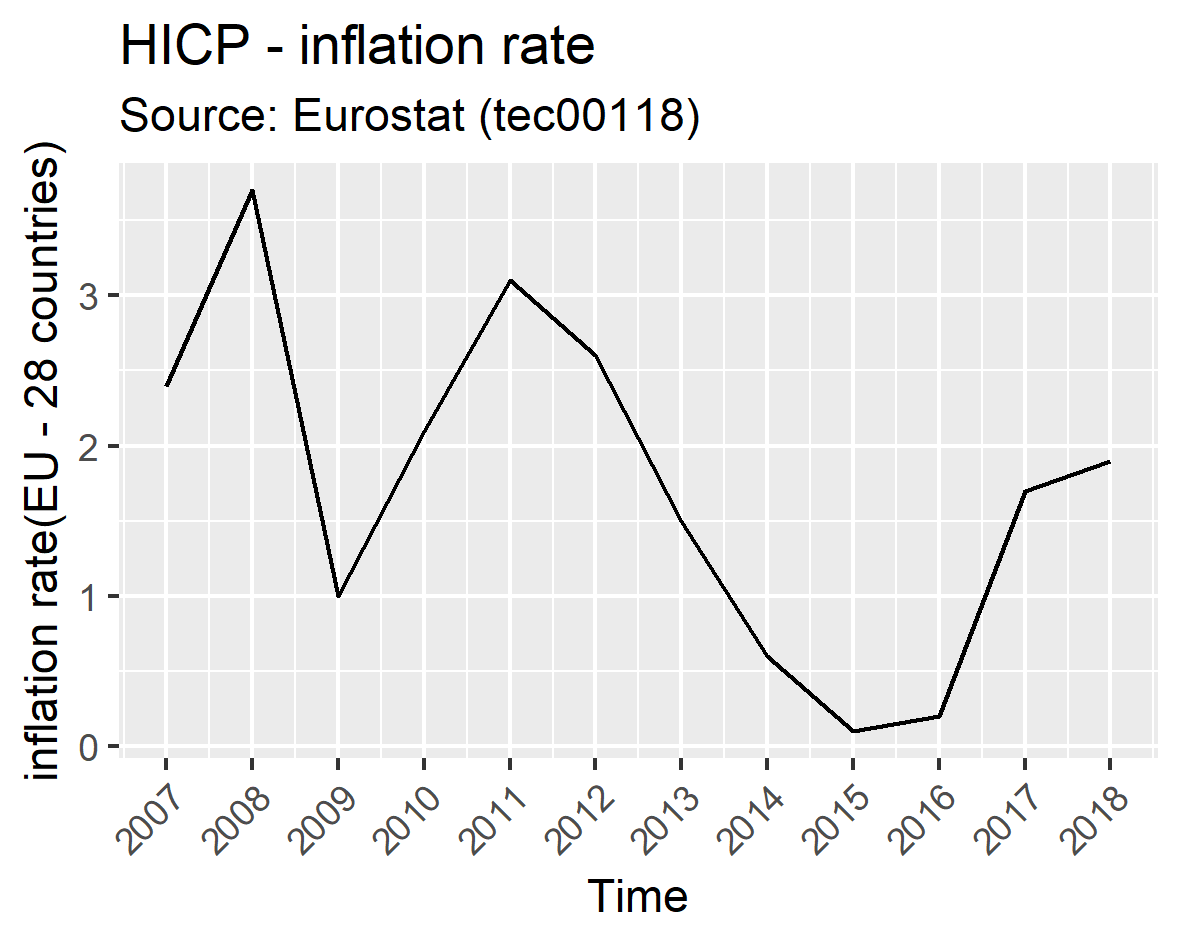
\includegraphics[width=.7\textwidth]{HICP.png}
    \caption{HICP - inflation rate}
    \label{figure 1}
\end{figure}


\end{document}
https://www.overleaf.com/project/5d04d45bf9cea35218a70433